% Springer Nature LaTeX Author Template
% Formatted specifically for submission to:
% Journal of Real-Time Image Processing (JRTIP), Springer Nature
%
\documentclass[pdflatex,sn-mathphys]{sn-jnl}

%%%% Standard Packages
\usepackage{graphicx}
\usepackage{multirow}
\usepackage{amsmath,amssymb,amsfonts}
\usepackage{amsthm}
\usepackage{mathrsfs}
\usepackage[title]{appendix}
\usepackage{xcolor}
\usepackage{textcomp}
\usepackage{manyfoot}
\usepackage{booktabs}
\usepackage{algorithm}
\usepackage{algorithmicx}
\usepackage{algpseudocode}
\usepackage{listings}
\usepackage{array}
\usepackage{url}
\def\UrlBreaks{\do\/\do-}
\usepackage{microtype}

\raggedbottom

\begin{document}

\title[Real-Time Attention-Guided Object Detection for Dense Unstructured Traffic]{Real-Time Attention-Guided Object Detection and Dynamic Feature Fusion for Dense Unstructured Traffic in Developing Regions}

%%=============================================================%%
%% Authors and Affiliations
%%=============================================================%%

\author[1]{\fnm{Md. Taher Bin Omar} \sur{Hijbullah}}
\author[1]{\fnm{Md. Rony} \sur{Mia}}
\author*[1]{\fnm{Mahedi} \sur{Hasan}}\email{mahedi.hasan@iubat.edu}
\author[1]{\fnm{Md. Rashedul} \sur{Islam}}
\author[1]{\fnm{Utpal Kanti} \sur{Das}}

\affil*[1]{\orgdiv{Department of Computer Science and Engineering}, \orgname{IUBAT---International University of Business Agriculture and Technology}, \orgaddress{\street{4 Embankment Drive Road, Sector 10, Uttara}, \city{Dhaka}, \postcode{1230}, \country{Bangladesh}}}

%%=============================================================%%
%% Abstract
%%=============================================================%%

\abstract{Automated visual perception is an important technology for Intelligent Transportation Systems (ITS) and Advanced Driver Assistance Systems (ADAS). However, high-performing vision models often lack reliability when transferred to the overcrowded streets of South Asian megacities, which are unstructured and exceedingly chaotic. The traffic composition on the roadways of Bangladesh is remarkably heterogeneous, characterized by a complete lack of lane discipline, extreme visual occlusion, and severe class imbalance, where high-speed motorized vehicles share space with low-speed non-motorized transports such as human-powered rickshaws, vans, and three-wheeled auto-rickshaws (CNGs). To address these perception gaps, this study presents an enhanced and optimized YOLOv11 framework capable of superior real-time performance even in complex urban traffic scenarios at the edge. We introduce two cooperative architectural improvements: (i) an optimized Convolutional Block Attention Module (CBAM) embedded into the deep feature extraction stage (Layer 23, P5 feature map), which sequentially reweights channel and spatial saliency, effectively suppresses background visual clutter, and sharpens the structural boundaries of occluded vehicles; and (ii) a Dynamic Channel Fusion Module (DCFM) with parallel multi-scale convolutional receptive fields and adaptive feature weighting to resolve scale disparities between diminutive and bulky road participants. We assembled multiple regional data sources to create a multi-source regional benchmark of nine localized classes, comprising 265,698 high-quality annotated bounding boxes across 23,648 images, strictly partitioned on a video level across 4,729 validation frames to eliminate temporal data leakage. Across extensive ablation experiments over 50 epochs, our attention-guided YOLOv11m architecture demonstrates outstanding performance on the visually challenging Rickshaw class with 90.8\% mAP@0.50 and improves the accuracy of the minority Truck class by +1.50\%, all with just a +0.16\% parameter overhead (+32,866 parameters). Even more significantly, the model achieves an ultra-low pure inference latency of 4.7~ms per frame ($\sim$212.7 FPS on an NVIDIA Tesla T4 GPU) due to attention-guided background suppression reducing non-maximum suppression (NMS) candidate queues. Furthermore, an extensive error analysis of cross-class structural confusion reveals that for severely underrepresented long-tail minority classes (e.g., Cycles), architectural enhancements alone cannot overcome absolute sample scarcity, establishing fundamental empirical guidelines for future ITS dataset curation. Finally, a containerized edge deployment prototype was validated, confirming the operational feasibility of scalable smart-city traffic monitoring.}

\keywords{Real-time object detection, YOLOv11, Convolutional Block Attention Module (CBAM), Dynamic Channel Fusion Module (DCFM), Unstructured traffic, Intelligent Transportation Systems (ITS), Edge-grade latency, Class imbalance}

\maketitle

%%=============================================================%%
%% Section 1: Introduction
%%=============================================================%%
\section{Introduction}\label{sec:intro}

In modern Intelligent Transportation Systems (ITS) and Advanced Driver Assistance Systems (ADAS), accurate and real-time computer vision techniques that provide perception of road dynamics, automated collision avoidance, and enforcement of civic road traffic rules play a pivotal role~\cite{geiger2012are,cordts2016cityscapes,redmon2016you,zhao2024detrs}. Highways and urban roadways in canonical object detection benchmarks---such as KITTI~\cite{geiger2012are} and Cityscapes~\cite{cordts2016cityscapes} in Western nations, as well as BDD100K and MS COCO~\cite{lin2014microsoft}---feature well-engineered geometries, regular lane widths, uniform asphalt striping, and standardized vehicle body morphologies. Consequently, convolutional object detectors engineered and validated exclusively on these conventional datasets develop strong spatial priors that presume highly regulated vehicular movements.

However, when these perception systems are deployed on the sprawling urban thoroughfares of developing South Asian nations, their performance degrades markedly due to extreme domain divergence, particularly within megacities such as Dhaka, Bangladesh~\cite{hasan2021bangladeshi,rahman2022fine,varma2019idd,hijbullah2026attention}. The traffic environments on Bangladeshi roadways represent an extreme manifestation of unstructured traffic dynamics. Rather than adhering to delimited road corridors, vehicular participants maneuver opportunistically and in an uncoordinated manner within shared physical road space. Crucially, modal composition is inherently heterogeneous: heavy industrial transit (e.g., long-distance buses and inter-district cargo trucks) shares the same lane space with compact motorized vehicles (private sedans, microbuses), intermediate three-wheelers (compressed natural gas auto-rickshaws, locally termed `CNG', and battery-powered `easy-bikes'), and highly vulnerable non-motorized transport modes (human-pedaled cycle rickshaws, flatbed freight vans, and unsegregated pedestrian clusters)~\cite{hossain2024visual,rahman2021densely}.

\begin{figure*}[t]
\centering
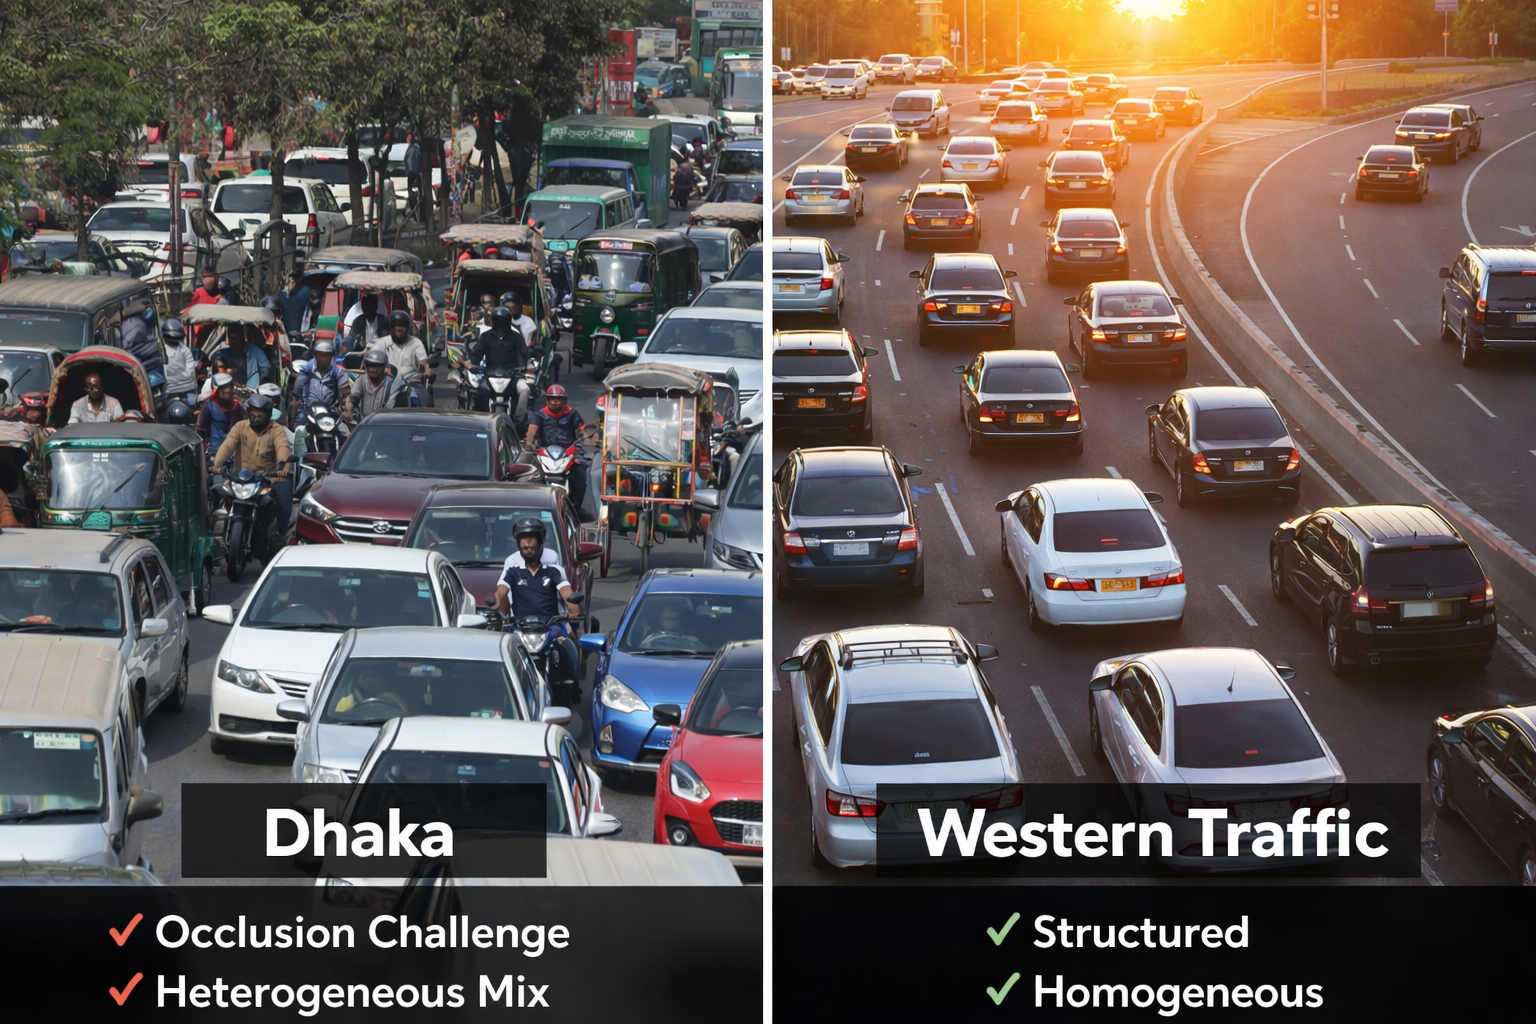
\includegraphics[width=0.95\textwidth]{figures/fig1_western_vs_dhaka.png}
\caption{Visual comparison highlighting structural domain divergence between canonical Western highway environments (exhibiting standardized vehicle models and strict lane adherence) and unstructured Dhaka traffic (characterized by heterogeneous multimodal vehicles, extreme proximity, and severe visual occlusion).}\label{fig:western_vs_dhaka}
\end{figure*}

As illustrated in Fig.~\ref{fig:western_vs_dhaka}, vehicles in dense operational regimes operate in close physical proximity, such that only fractured segments of their structures are visible from roadside or onboard cameras, creating conditions of extreme visual occlusion. When background clutter and adjacent vehicular textures merge into a monolithic feature representation, standard deep backbones generate ambiguous candidate predictions, confusing non-maximum suppression (NMS) thresholds into deleting valid bounding boxes or misassigning boundaries. Furthermore, roadway entities exhibit vast dimensional variance, spanning high-chassis passenger buses down to skeletal, human-pedaled bicycles. Conventional convolutional receptive fields frequently struggle to simultaneously capture the global context of large commercial vehicles while preserving the subtle, thin metallic contours of small, low-profile two-wheelers.

To address these intertwined perception bottlenecks, this study presents an attention-guided real-time perception architecture built upon the latest YOLOv11 framework~\cite{jocher2024yolo11,khanam2024yolov11}. The primary contributions of this paper are summarized as follows:
\begin{itemize}
    \item \textbf{Architectural Innovation with Zero Latency Penalty:} We propose a customized YOLOv11m architecture that injects a Convolutional Block Attention Module (CBAM)~\cite{woo2018cbam} specifically into the deep feature extraction stage (Layer 23, P5 feature map). This configuration suppresses background clutter and sharpens structural boundary saliency under extreme occlusion while adding merely 32,866 parameters (+0.16\% overhead) and achieving an inference latency of 4.7~ms per frame ($\sim$212.7 FPS on an NVIDIA Tesla T4 GPU), preserving edge-computing viability.
    
    \item \textbf{Dynamic Multi-Scale Feature Fusion:} Addressing the substantial scale disparities of vehicles in dense urban environments, we formulate and evaluate a Dynamic Channel Fusion Module (DCFM) equipped with parallel multi-scale convolutional receptive fields and learnable channel gating weights.
    
    \item \textbf{Unified Large-Scale Regional Benchmark:} We construct and standardize a curated multi-source benchmark comprising 265,698 annotated object instances across 23,648 high-resolution images, enforcing strict video-wise partitioning across 4,729 validation frames to eliminate temporal frame correlation and data leakage~\cite{islam2025bangladeshi,shihavuddin2020dhakaai,sujoy2024monocular}.
    
    \item \textbf{Empirical Discovery on Architectural Limits vs. Long-Tail Imbalance:} Through systematic quantitative benchmarking and confusion matrix isolation, we demonstrate that while architectural attention mechanisms significantly bolster detection for visually complex vehicles with moderate sample support (e.g., Rickshaws reaching 90.8\% mAP@0.50, Trucks gaining +1.50\%), architectural modifications alone cannot resolve severe minority-class collapse under extreme sample scarcity (e.g., Cycles), establishing foundational empirical guidelines for future ITS dataset curation.
    
    \item \textbf{Edge Deployment Prototype:} We validate the practical operational feasibility of the proposed attention-guided detector through a containerized Streamlit edge surveillance application capable of real-time stream processing at $>$200 FPS on GPU hardware.
\end{itemize}

The remainder of this paper is organized as follows: Section~\ref{sec:related} reviews related work on real-time detectors, visual attention mechanisms, and unstructured traffic datasets. Section~\ref{sec:method} details the mathematical formulation and proposed architecture. Section~\ref{sec:dataset} presents the dataset engineering pipeline and experimental setup. Section~\ref{sec:results} discusses ablation findings, convergence dynamics, and latency benchmarks. Section~\ref{sec:error} provides error isolation through confusion matrices. Section~\ref{sec:deployment} demonstrates the edge deployment prototype. Finally, Section~\ref{sec:discussion} discusses limitations and concludes the paper.

%%=============================================================%%
%% Section 2: Related Work
%%=============================================================%%
\section{Related Work}\label{sec:related}

\subsection{Evolution of Real-Time One-Stage Object Detectors}
The development of deep learning for object detection has changed drastically from computationally intensive two-stage methods to high-speed one-stage architectures~\cite{redmon2016you,ren2015faster,wang2023yolov7}. Two-stage detectors, typified by Faster R-CNN~\cite{ren2015faster}, generate sparse region proposals in the first stage, which are then regressed and classified in the second; while achieving high localization accuracy, they suffer from prohibitive computational latency that makes them unsuitable for real-time edge robotics. In a groundbreaking departure, Redmon et al.~\cite{redmon2016you} presented You Only Look Once (YOLO), reformulating object detection as a unified, single-shot spatial regression problem that directly predicts bounding box coordinates and class conditional probabilities from raw pixels.

Each successive generation of the YOLO family methodically worked to refine architectural elements. YOLOv4~\cite{bochkovskiy2020yolov4} incorporated CSPNet backbones, Path Aggregation Networks (PANet)~\cite{liu2018path}, and Mish activations. YOLOv7~\cite{wang2023yolov7} integrated extended efficient layer aggregation networks (E-ELAN). To maintain semantic signals across deep hierarchies, YOLOv9~\cite{wang2024yolov9} proposed programmable gradient information (PGI). YOLOv10~\cite{wang2024yolov10} introduced dual-label assignments for NMS-free inference. Recently, Ultralytics introduced YOLOv11~\cite{jocher2024yolo11}, featuring improved C3k2 building blocks, streamlined Cross Stage Partial connections, and Cross Stage Partial with Spatial Attention (C2PSA) modules to optimize deep gradient propagation and reduce parameter redundancy~\cite{khanam2024yolov11}. Meanwhile, real-time transformer models like RT-DETR~\cite{zhao2024detrs} have demonstrated competitive accuracy, but convolutional vision models remain superior in memory efficiency and edge deployment maturity. However, off-the-shelf YOLO detectors continue to exhibit notable recall drops when deployed in unstructured visual domains characterized by dense occlusions and non-canonical object geometries~\cite{hasan2021bangladeshi,rahman2021densely}.

\subsection{Visual Attention Mechanisms in Object Detection}
Visual attention mechanisms dynamically modulate neural feature responses, amplifying task-relevant feature dimensions while suppressing spatially or channel-wise irrelevant background noise~\cite{woo2018cbam,hu2018squeeze,wang2020eca,hou2021coordinate}. Although Hu et al.~\cite{hu2018squeeze} pioneered the Squeeze-and-Excitation (SE) network for channel-wise recalibration using global average pooling and multi-layer perceptron (MLP) gating, it inherently discarded critical spatial coordinates. To address this limitation, Wang et al.~\cite{wang2020eca} proposed ECA-Net, utilizing 1D convolutions to capture local cross-channel interaction without dimensionality reduction. Hou et al.~\cite{hou2021coordinate} formulated Coordinate Attention, embedding directional positional information into channel maps via 1D spatial pooling.

Woo et al.~\cite{woo2018cbam} proposed the Convolutional Block Attention Module (CBAM), sequentially cascading channel attention and spatial attention. CBAM simultaneously learns `what to focus on' and `where to focus' by combining both max-pooled and average-pooled spatial descriptors across a large $7\times 7$ receptive field. Tan et al.~\cite{tan2020efficientdet} highlighted the importance of weighted bidirectional feature network (BiFPN) fusion for multi-scale context. In recent years, attention mechanisms have been successfully deployed in specialized vision domains: Garshasebi~\cite{garshasebi2025improving} embedded CBAM into YOLO11 for small object detection in remote sensing imagery; Khan et al.~\cite{khan2025defect} applied attention-guided YOLOv11 for defect detection on industrial surfaces; and Zhang et al.~\cite{zhang2025trinext} developed TriNext, a three-path multi-scale feature enhancement module. However, systematically introducing sequential spatial-channel attention into deep feature hierarchies for dense, mixed non-motorized urban traffic remains largely unexplored.

\subsection{Traffic Object Detection in Unstructured Developing Environments}
Traffic patterns in the urban corridors of developing South Asian economies depart fundamentally from Western driving regimes~\cite{hasan2021bangladeshi,rahman2022fine,varma2019idd}. ITS solutions in Western countries presume clear lane lines, vehicle homogeneity (cars, trucks, motorcycles), and uniform speed profiles. Road corridors in megacities such as Dhaka, Bangladesh, by contrast, are characterized by extreme modal heterogeneity: high-speed transit buses intermingle with non-motorized pedal rickshaws, auto-rickshaws (CNGs), freight vans, and unsegregated pedestrians~\cite{hossain2024visual,rahman2021densely}.

To encourage research, several regional datasets have been released, including the Mendeley Bangladeshi Traffic Flow Dataset~\cite{islam2025bangladeshi}, the DhakaAI dataset~\cite{shihavuddin2020dhakaai}, the Poribohon-BD dataset~\cite{sujoy2024monocular}, and the India Driving Dataset (IDD)~\cite{varma2019idd}. Early studies by Hasan et al.~\cite{hasan2021bangladeshi} and Rahman et al.~\cite{rahman2022fine} utilized transfer learning on standard CNNs for localized vehicle classification but did not address dense bounding-box object detection or real-time edge constraints. Rahman et al.~\cite{rahman2021densely} explored YOLOv5 ensembles for dense traffic, yet their approach incurred prohibitive computational overhead that precluded edge deployment. Crucially, previous benchmarks have frequently relied on random train-test frame shuffling, resulting in severe temporal data leakage across sequential video frames. In this work, we tackle these shortcomings by introducing a unified, video-partitioned regional benchmark and an attention-guided architecture optimized for edge-grade execution.

%%=============================================================%%
%% Section 3: Proposed Methodology
%%=============================================================%%
\section{Proposed Methodology and Mathematical Formulation}\label{sec:method}

This section presents the architectural foundation and mathematical formulation of our proposed framework, delineating the baseline YOLOv11 multi-task loss formulation, the strategic integration of the Convolutional Block Attention Module (CBAM) within deep backbone hierarchies, and the design of the Dynamic Channel Fusion Module (DCFM).

\subsection{Baseline YOLOv11 Formulation and Multi-Task Loss Objectives}\label{subsec:loss}

The baseline YOLOv11 architecture processes an input image $I \in \mathbb{R}^{3 \times H_{in} \times W_{in}}$ through a multi-stage convolutional backbone to construct hierarchical feature pyramids denoting spatial strides $\{P_3, P_4, P_5\}$, corresponding to downsampling factors of 8, 16, and 32, respectively. The detection head employs decoupled branches for bounding box regression and class probability estimation.

The multi-task optimization objective combines Complete Intersection over Union (CIoU) loss~\cite{zheng2020distance,gevorgyan2022siou}, Distribution Focal Loss (DFL)~\cite{li2020generalized}, and Binary Cross-Entropy (BCE) classification loss~\cite{zhang2021varifocalnet}:
\begin{equation}
\mathcal{L}_{\text{total}} = \lambda_{\text{box}} \mathcal{L}_{\text{CIoU}} + \lambda_{\text{dfl}} \mathcal{L}_{\text{DFL}} + \lambda_{\text{cls}} \mathcal{L}_{\text{cls}}
\label{eq:total_loss}
\end{equation}
where $\lambda_{\text{box}} = 7.5$, $\lambda_{\text{dfl}} = 1.5$, and $\lambda_{\text{cls}} = 0.5$ denote task balancing weights.

The CIoU loss evaluates three distinct geometric factors: overlap area, Euclidean distance between center points, and aspect ratio alignment:
\begin{equation}
\mathcal{L}_{\text{CIoU}} = 1 - \text{IoU} + \frac{\rho^2(\mathbf{b}, \mathbf{b}_{\text{gt}})}{c^2} + \alpha v
\label{eq:ciou}
\end{equation}
where $\mathbf{b} = [x, y, w, h]$ and $\mathbf{b}_{\text{gt}} = [x_{\text{gt}}, y_{\text{gt}}, w_{\text{gt}}, h_{\text{gt}}]$ represent the central coordinates and dimensions of the predicted and ground-truth bounding boxes, respectively; $\rho(\cdot)$ denotes Euclidean distance; $c$ is the diagonal length of the smallest enclosing bounding box covering both objects; and $v$ measures aspect ratio consistency:
\begin{equation}
v = \frac{4}{\pi^2} \left( \arctan\frac{w_{\text{gt}}}{h_{\text{gt}}} - \arctan\frac{w}{h} \right)^2
\label{eq:v}
\end{equation}
The parameter $\alpha$ is a dynamic weighting factor defined as:
\begin{equation}
\alpha = \frac{v}{(1 - \text{IoU}) + v}
\label{eq:alpha}
\end{equation}

To capture fine-grained localization uncertainty under severe occlusion, Distribution Focal Loss (DFL) models continuous regression coordinates as a general probability distribution over discrete bins. Rather than predicting a single deterministic coordinate value, DFL models a flexible representation of bounding box boundaries by weighting the probability of adjacent discrete indices:
\begin{equation}
\mathcal{L}_{\text{DFL}}(S_i, S_{i+1}) = - \Big( (y_{i+1} - y)\log(S_i) + (y - y_i)\log(S_{i+1}) \Big)
\label{eq:dfl}
\end{equation}
where $y$ is the continuous ground-truth coordinate, $y_i$ and $y_{i+1}$ are adjacent discrete grid indices ($y_i \le y \le y_{i+1}$), and $S_i, S_{i+1}$ denote the softmax outputs of the regression network.

The classification loss $\mathcal{L}_{\text{cls}}$ is formulated via Binary Cross-Entropy loss across all $C=9$ vehicular categories, penalizing predicted class probability deviations against ground-truth binary indicators:
\begin{equation}
\mathcal{L}_{\text{cls}} = - \sum_{c=1}^{C} \Big( y_c \log(p_c) + (1 - y_c)\log(1 - p_c) \Big)
\label{eq:bce}
\end{equation}
where $y_c \in \{0, 1\}$ is the class label and $p_c \in [0, 1]$ represents the predicted class probability.

\subsection{Strategic CBAM Integration at Deep Feature Stage (Layer 23)}\label{subsec:cbam}

Visual occlusion manifests as a critical challenge in the congested traffic of South Asia, where large buses and trucks conceal adjacent smaller vehicles such as rickshaws and bicycles. However, high-level semantic feature maps in standard convolutional backbones suffer from spatial ambiguities: as receptive fields expand, object boundaries blur into adjacent background textures, causing feature corruption. To resolve this limitation, we incorporate a customized Convolutional Block Attention Module (CBAM)~\cite{woo2018cbam} directly into Layer 23 of the YOLOv11m backbone, intercepting the 512-channel $P_5$ feature map immediately prior to the multi-scale detection neck.

\begin{figure*}[t]
\centering
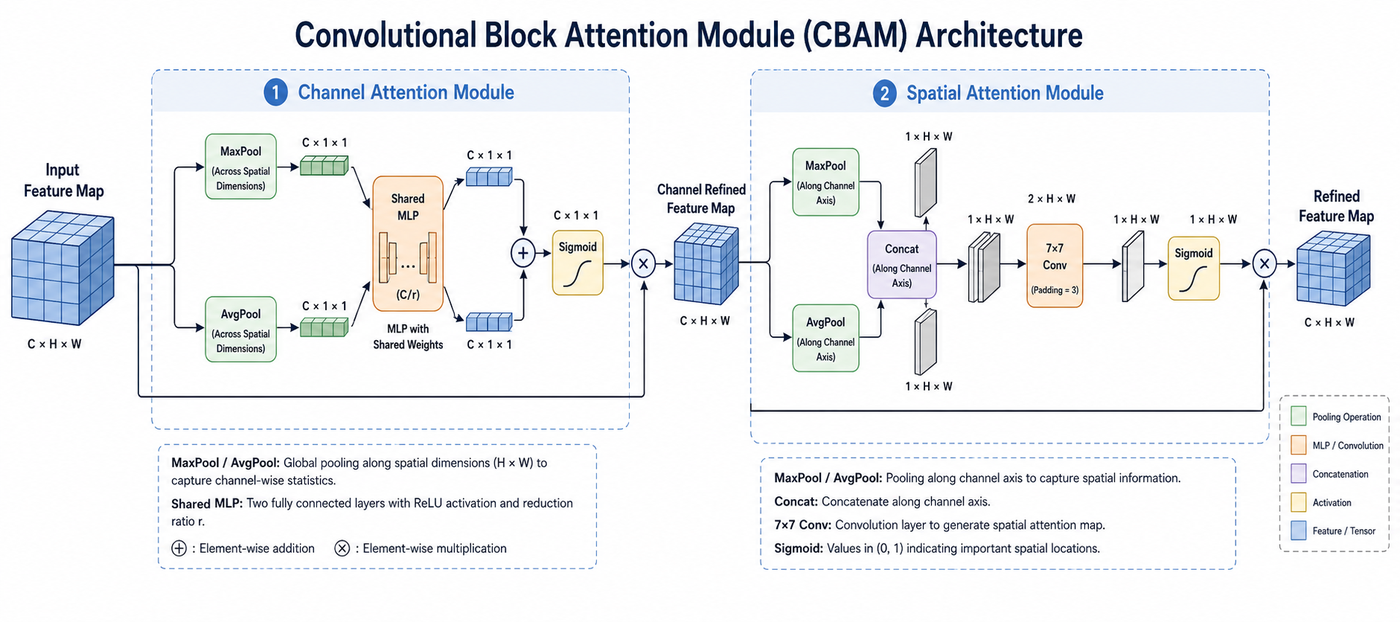
\includegraphics[width=0.90\textwidth]{figures/fig2_cbam_architecture.png}
\caption{Schematic architecture of the Convolutional Block Attention Module (CBAM), detailing the sequential channel attention and spatial attention recalibration sub-modules.}\label{fig:cbam_arch}
\end{figure*}

As illustrated in Fig.~\ref{fig:cbam_arch}, the module executes a sequential two-step recalibration process on intermediate feature tensor $\mathbf{F} \in \mathbb{R}^{C \times H \times W}$ ($C=512$).

\textbf{1. Channel Attention Sub-Module:} Spatial dimensions are compressed using parallel Global Average Pooling and Global Max Pooling operations to aggregate diverse spatial context descriptors:
\begin{align}
\mathbf{F}_{\text{avg}}^c &= \text{AvgPool}(\mathbf{F}) \in \mathbb{R}^{C \times 1 \times 1} \\
\mathbf{F}_{\text{max}}^c &= \text{MaxPool}(\mathbf{F}) \in \mathbb{R}^{C \times 1 \times 1}
\end{align}
Both descriptors are forwarded through a shared multi-layer perceptron (MLP) with a reduction ratio $r=16$. The channel attention map $\mathbf{M}_c \in \mathbb{R}^{C \times 1 \times 1}$ is produced via element-wise summation and sigmoid activation:
\begin{equation}
\mathbf{M}_c(\mathbf{F}) = \sigma \Big( \mathbf{W}_1 \cdot \text{ReLU}(\mathbf{W}_0 \cdot \mathbf{F}_{\text{avg}}^c) + \mathbf{W}_1 \cdot \text{ReLU}(\mathbf{W}_0 \cdot \mathbf{F}_{\text{max}}^c) \Big)
\label{eq:channel_att}
\end{equation}
where $\mathbf{W}_0 \in \mathbb{R}^{(C/r) \times C}$ and $\mathbf{W}_1 \in \mathbb{R}^{C \times (C/r)}$ denote the shared MLP weights, and $\sigma$ represents the sigmoid function. The channel-recalibrated feature map $\mathbf{F}'$ is obtained via channel-wise multiplication:
\begin{equation}
\mathbf{F}' = \mathbf{M}_c(\mathbf{F}) \otimes \mathbf{F}
\label{eq:channel_mult}
\end{equation}

\textbf{2. Spatial Attention Sub-Module:} Channel descriptors are aggregated along the channel dimension using average and max pooling operations to generate informative 2D spatial maps:
\begin{equation}
\mathbf{M}_s(\mathbf{F}') = \sigma \left( f^{7\times 7} \left( \big[ \text{AvgPool}_c(\mathbf{F}') \;;\; \text{MaxPool}_c(\mathbf{F}') \big] \right) \right)
\label{eq:spatial_att}
\end{equation}
where $[\cdot \,;\, \cdot]$ denotes channel-wise concatenation, and $f^{7\times 7}$ represents a convolutional operation with a $7\times 7$ kernel filter. The finalized attention-enhanced feature tensor $\mathbf{F}''$ is computed as:
\begin{equation}
\mathbf{F}'' = \mathbf{M}_s(\mathbf{F}') \otimes \mathbf{F}'
\label{eq:spatial_mult}
\end{equation}

\begin{figure*}[t]
\centering
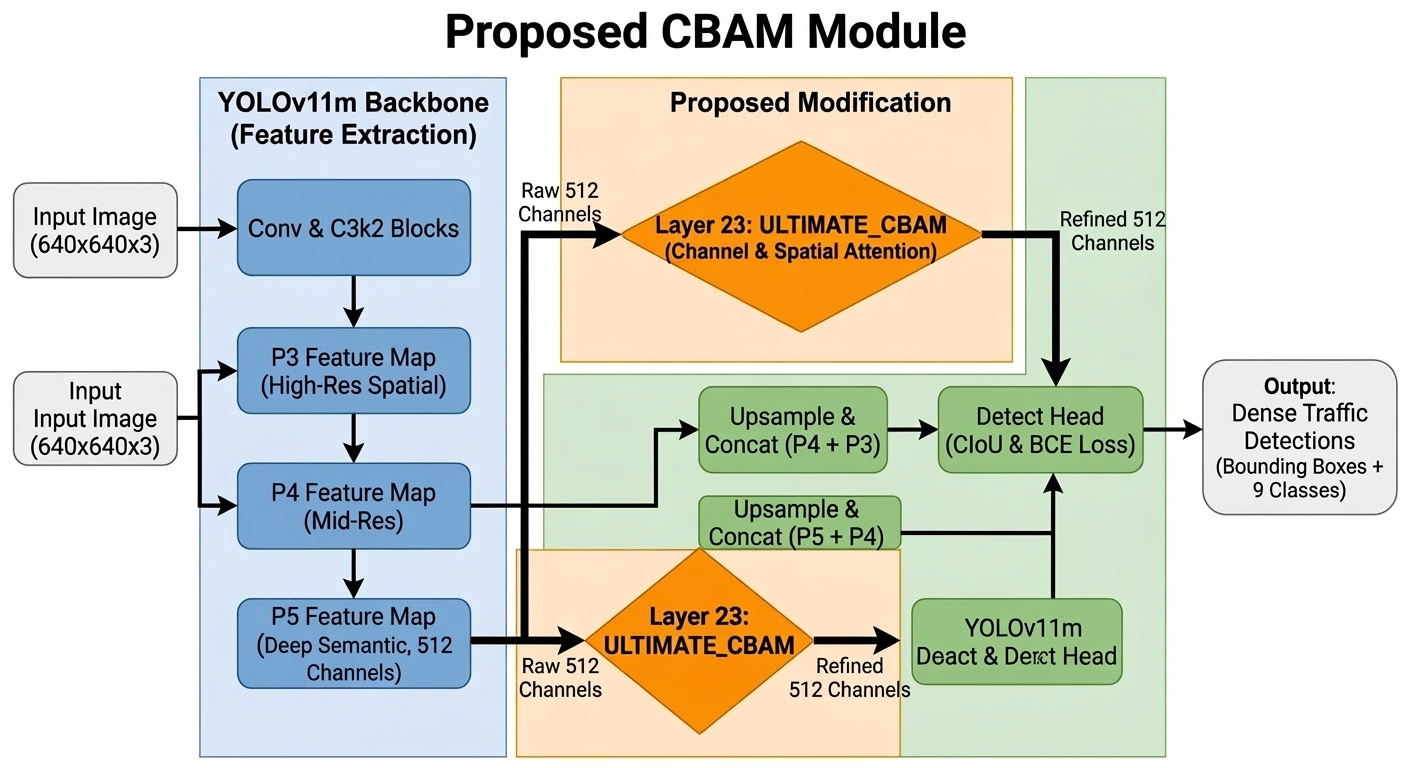
\includegraphics[width=0.98\textwidth]{figures/fig3_proposed_pipeline.png}
\caption{Complete architectural pipeline of the proposed Attention-Guided YOLOv11m framework, showing the exact point of CBAM injection at Layer 23 intercepting the 512-channel P5 feature map.}\label{fig:proposed_pipeline}
\end{figure*}

Fig.~\ref{fig:proposed_pipeline} depicts the end-to-end integration within the YOLOv11m architecture. Injecting CBAM precisely at Layer 23 filters out non-informative road asphalt and sky clutter at the deepest semantic level before neck aggregation, sharpening the contours and boundary edges of vehicles in heavily occluded traffic.

\subsection{Dynamic Channel Fusion Module (DCFM)}\label{subsec:dcfm}

To resolve extreme vehicle scale disparities where diminutive pedal bicycles coexist with large inter-district buses, we developed the Dynamic Channel Fusion Module (DCFM). Rather than relying on static feature concatenation, DCFM routes input feature maps to parallel multi-scale convolutional operations and applies dynamic softmax gating across receptive fields.

\begin{figure*}[t]
\centering
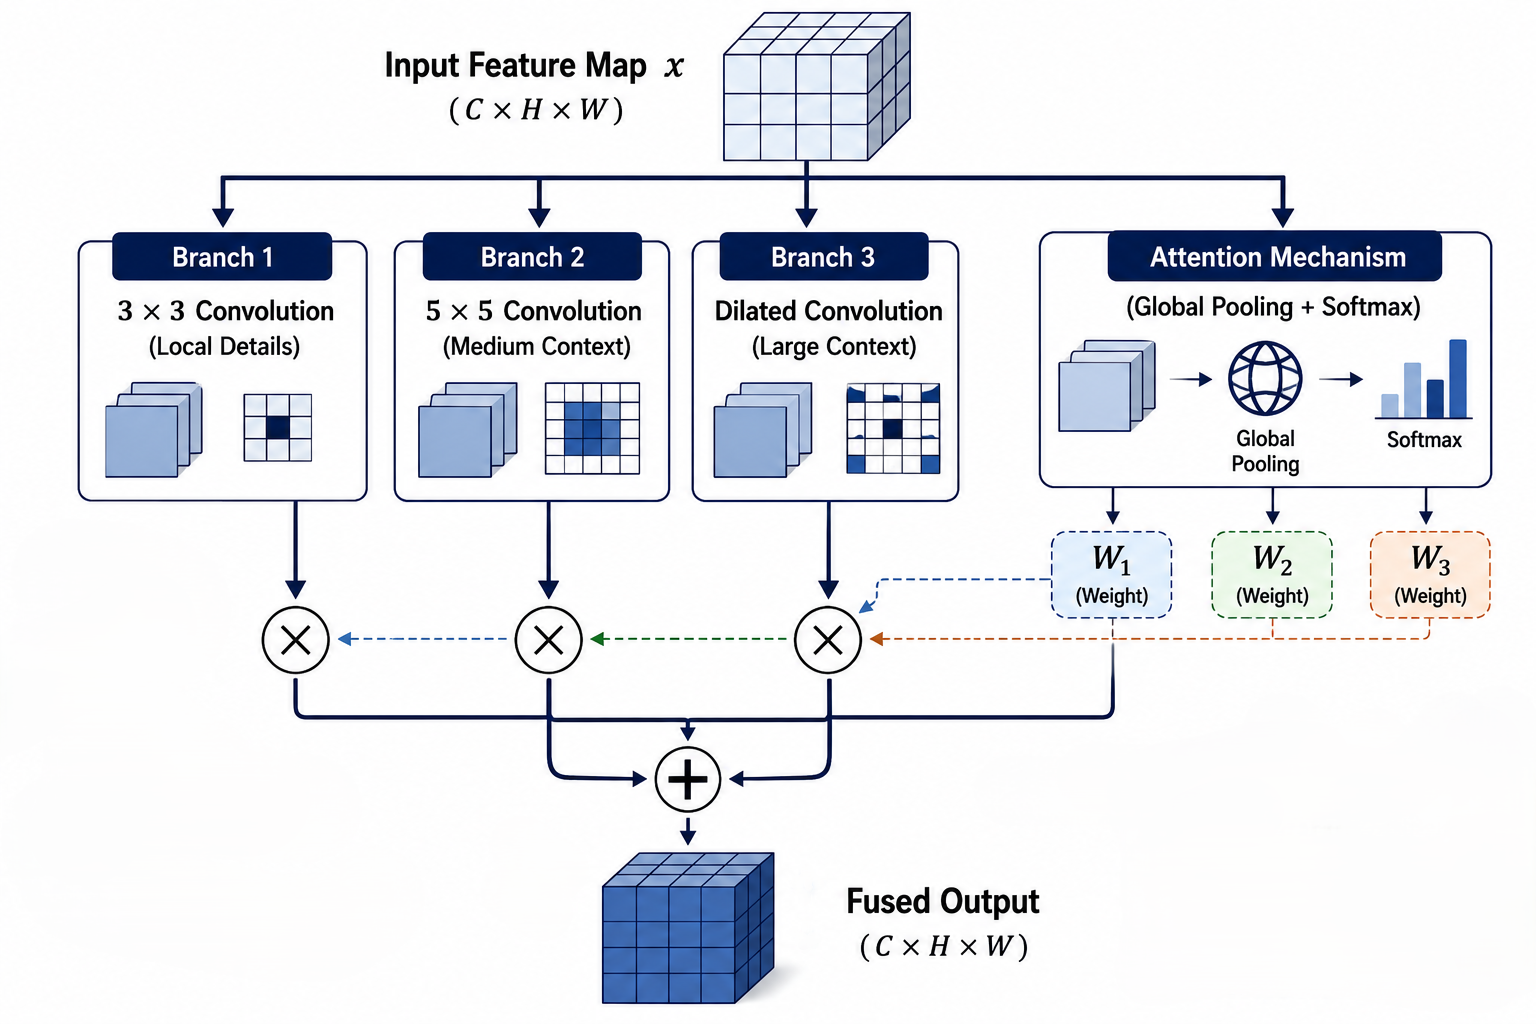
\includegraphics[width=0.90\textwidth]{figures/fig4_dcfm_architecture.png}
\caption{Architecture of the Dynamic Channel Fusion Module (DCFM), illustrating parallel multi-scale convolutional branches and learnable dynamic channel gating.}\label{fig:dcfm_arch}
\end{figure*}

As shown in Fig.~\ref{fig:dcfm_arch}, given an input feature tensor $\mathbf{F} \in \mathbb{R}^{C \times H \times W}$, DCFM employs $K$ parallel convolutional branches with diverse kernel sizes and dilation rates $\{d_1, d_2, \dots, d_K\}$ to extract multi-scale receptive field descriptors:
\begin{equation}
\mathbf{U}_k = \text{Conv}_k(\mathbf{F}), \quad k \in \{1, 2, \dots, K\}
\end{equation}
Global contextual statistics are aggregated using Global Average Pooling (GAP) across the spatial dimensions:
\begin{equation}
\mathbf{s} = \text{GAP}(\mathbf{F}) = \frac{1}{H \times W} \sum_{i=1}^{H} \sum_{j=1}^{W} \mathbf{F}(:, i, j)
\end{equation}
A lightweight gating network computes learnable adaptive attention weights $\boldsymbol{\alpha} = [\alpha_1, \alpha_2, \dots, \alpha_K]$ via softmax normalization across all branches:
\begin{equation}
\alpha_k = \frac{\exp(\mathbf{W}_k \cdot \mathbf{s})}{\sum_{j=1}^{K} \exp(\mathbf{W}_j \cdot \mathbf{s})}, \quad \sum_{k=1}^{K} \alpha_k = 1
\label{eq:dcfm_gate}
\end{equation}
where $\mathbf{W}_k \in \mathbb{R}^{C \times C}$ denotes the parameter matrix for branch $k$. The dynamically fused feature tensor $\mathbf{F}_{\text{DCFM}}$ is synthesized through weighted feature integration:
\begin{equation}
\mathbf{F}_{\text{DCFM}} = \sum_{k=1}^{K} \alpha_k \otimes \mathbf{U}_k
\label{eq:dcfm_fuse}
\end{equation}
This formulation empowers the network to adaptively adjust receptive field weights based on the instantaneous scale composition of detected traffic participants.

%%=============================================================%%
%% Section 4: Dataset Engineering & Setup
%%=============================================================%%
\section{Dataset Engineering and Experimental Setup}\label{sec:dataset}

\subsection{Curated Benchmark Dataset Construction}
To establish an authoritative empirical benchmark for unstructured traffic perception, we curated a unified regional dataset by harmonizing images and annotations from three publicly accessible repositories:
\begin{enumerate}
    \item \textbf{Mendeley Bangladeshi Traffic Flow Dataset}~\cite{islam2025bangladeshi}: Providing high-density multi-angle urban corridor recordings across diverse weather and lighting conditions.
    \item \textbf{DhakaAI Autonomous Driving Dataset}~\cite{shihavuddin2020dhakaai}: Providing dashcam and roadside perspectives captured in core metropolitan Dhaka.
    \item \textbf{Poribohon-BD Dataset}~\cite{sujoy2024monocular}: Providing monocular irregular traffic instances featuring local non-motorized vehicles.
\end{enumerate}

All disparate annotation formats (Pascal VOC XML, COCO JSON) were cleaned, verified, and converted to a standardized YOLO bounding box coordinate format:
\begin{equation}
[x_{\text{center}}, y_{\text{center}}, w, h] \in [0, 1]^4
\end{equation}
The finalized unified benchmark comprises 23,648 high-resolution images and 265,698 meticulously curated and verified instances spanning nine localized vehicle classes.

\begin{figure*}[t]
\centering
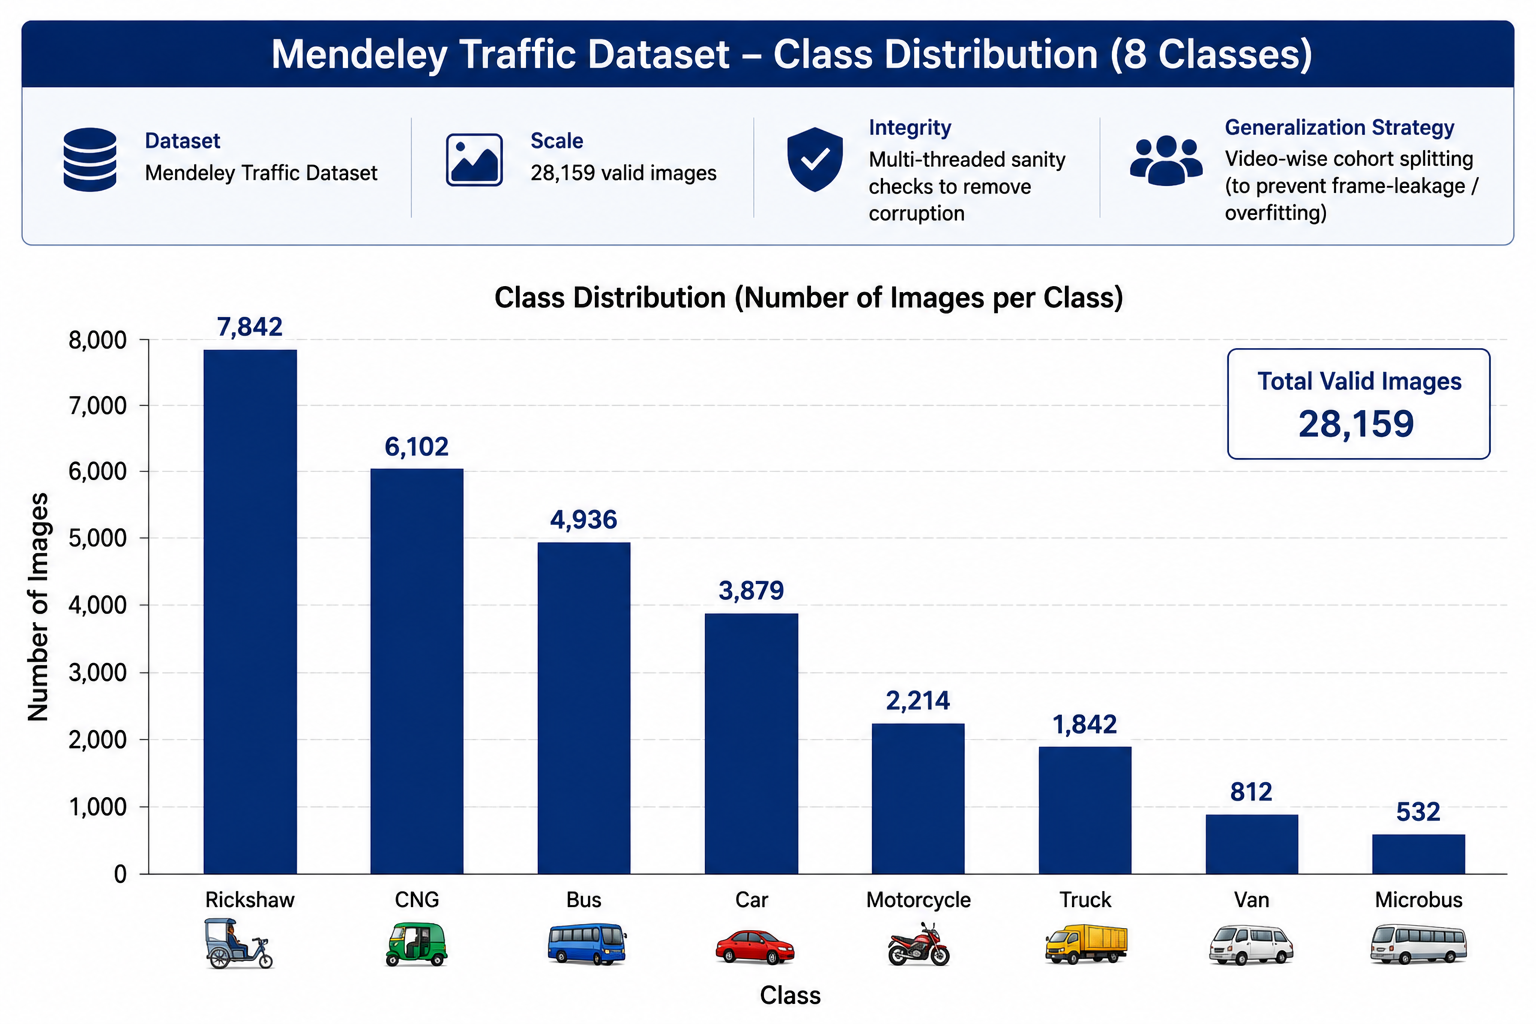
\includegraphics[width=0.92\textwidth]{figures/fig5_dataset_distribution.png}
\caption{Distribution of object instances across the nine regional traffic classes, demonstrating the severe long-tailed imbalance characteristic of South Asian road environments.}\label{fig:dataset_dist}
\end{figure*}

As illustrated in Fig.~\ref{fig:dataset_dist}, the vehicular frequency exhibits a steep long-tailed distribution. We categorize the nine classes into three distinct frequency tiers:
\begin{itemize}
    \item \textbf{Dominant Classes ($>$50k instances):} Car (63,107; 23.75\%), Rickshaw (60,241; 22.67\%), Bus (51,996; 19.57\%).
    \item \textbf{Mid-Tier Classes (10k--50k instances):} People / Pedestrian (38,779; 14.59\%), CNG / Auto-rickshaw (27,823; 10.47\%), Bike / Motorcycle (15,894; 5.98\%).
    \item \textbf{Minority Classes ($<$10k instances):} Mini-Truck (5,834; 2.20\%), Truck (1,310; 0.49\%), Cycle / Bicycle (714; 0.27\%).
\end{itemize}

Table~\ref{tab:dataset_distribution} summarizes the instance counts across training and validation partitions.

\begin{table*}[t]
\caption{Distribution of Annotated Vehicle Instances in the Curated Benchmark Dataset}\label{tab:dataset_distribution}
\resizebox{\textwidth}{!}{%
\begin{tabular}{llrrr}
\toprule
Class Tier & Vehicle Class & Training Instances & Validation Instances & Total Instances (Share) \\
\midrule
\multirow{3}{*}{Dominant ($>$50k)} 
 & Car & 50,584 & 12,523 & 63,107 (23.75\%) \\
 & Rickshaw (Non-motorized) & 48,357 & 11,884 & 60,241 (22.67\%) \\
 & Bus & 41,573 & 10,423 & 51,996 (19.57\%) \\
\midrule
\multirow{3}{*}{Mid-Tier (10k--50k)} 
 & People (Pedestrian) & 30,924 & 7,855 & 38,779 (14.59\%) \\
 & CNG (Auto-rickshaw) & 22,356 & 5,467 & 27,823 (10.47\%) \\
 & Bike (Motorcycle) & 12,740 & 3,154 & 15,894 (5.98\%) \\
\midrule
\multirow{3}{*}{Minority ($<$10k)} 
 & Mini-Truck & 4,647 & 1,187 & 5,834 (2.20\%) \\
 & Truck & 1,009 & 301 & 1,310 (0.49\%) \\
 & Cycle (Bicycle) & 566 & 148 & 714 (0.27\%) \\
\midrule
\textbf{Aggregate} & \textbf{All 9 Classes} & \textbf{212,756 (80.08\%)} & \textbf{52,942 (19.92\%)} & \textbf{265,698 (100.0\%)} \\
\bottomrule
\end{tabular}%
}
\end{table*}

\subsection{Video-Wise Sequence Partitioning}
A major pitfall in published traffic detection literature is the reliance on random frame-level shuffling. In video-based datasets, adjacent frames extracted at 30 FPS share near-identical background geometry, lighting conditions, and vehicular positions. Random frame partitioning results in substantial information leakage, artificially inflating reported validation accuracy.

To prevent this data leakage, we enforced strict video-wise sequence partitioning. Continuous frame sequences belonging to a particular camera stream or recording session were assigned exclusively to either the training set (80\%, 18,919 images) or the validation set (20\%, 4,729 images containing 52,941 ground-truth instances). Consequently, validation frames depict entirely unseen roadway scenes, ensuring authentic generalizability testing.

\subsection{Experimental Environment and Hyperparameter Configuration}
All models were implemented in PyTorch using the Ultralytics framework and trained on a dedicated computing cluster equipped with dual NVIDIA Tesla T4 GPUs (16~GB GDDR6 VRAM each, 32~GB aggregate). 

The experimental training hyperparameters were configured as follows:
\begin{itemize}
    \item Input Image Resolution: $640 \times 640$ pixels (with high-resolution benchmarking at $1280 \times 1280$ for YOLO26m).
    \item Training Epochs: 50 epochs with early stopping monitoring validation mAP.
    \item Batch Size: 32 distributed across dual GPUs.
    \item Optimizer: Stochastic Gradient Descent (SGD) with initial learning rate $\eta_0 = 0.01$, final learning rate factor $0.01$, momentum $0.937$, and weight decay $0.0005$.
    \item Learning Rate Schedule: Cosine annealing scheduler with a 3-epoch linear warmup period.
    \item Precision: Automatic Mixed Precision (AMP FP16) to accelerate computation and optimize memory bandwidth.
    \item Data Augmentation: Mosaic augmentation, random horizontal flipping ($p=0.5$), HSV color jittering, and affine translation ($\pm 0.1$).
\end{itemize}

%%=============================================================%%
%% Section 5: Results & Discussion
%%=============================================================%%
\section{Experimental Results and Comparative Analysis}\label{sec:results}

\subsection{Comprehensive Architectural Ablation and Latency Benchmarking}
To validate the efficacy of our proposed modifications, we conducted extensive ablation benchmarking across five architectural configurations: the baseline YOLOv11m, the multi-scale YOLOv11m + DCFM, the proposed attention-guided YOLOv11m + CBAM, the YOLO26m baseline, and the high-resolution YOLO26m variant ($1280 \times 1280$).

Table~\ref{tab:ablation} details the comprehensive quantitative findings, evaluating model parameter counts, floating-point operations (GFLOPs), mean Average Precision at IoU thresholds of 0.50 (mAP@0.50) and 0.50:0.95 (mAP@0.50:0.95), global recall, per-frame latency breakdown (preprocessing, neural inference, and postprocessing), and operational throughput (frames per second).

\begin{table*}[t]
\caption{Comprehensive Architectural Ablation, Computational Complexity, and Latency Breakdown}\label{tab:ablation}
\resizebox{\textwidth}{!}{%
\begin{tabular}{lccccccccc}
\toprule
Model Configuration & Params & GFLOPs & mAP@50 & mAP@50:95 & Recall & Pre (ms) & Infer (ms) & Post (ms) & FPS \\
\midrule
YOLOv11m Baseline & 20.04M & 67.7 & 75.10\% & 52.80\% & 71.40\% & 0.1 & 5.0 & 0.6 & 200.0 \\
YOLOv11m + DCFM & 20.21M & 69.4 & 74.80\% & 52.40\% & \textbf{73.10\%} & 0.1 & 5.3 & 0.6 & 188.7 \\
\textbf{YOLOv11m + CBAM (Proposed)} & \textbf{20.07M} & \textbf{67.7} & \textbf{75.70\%} & \textbf{53.20\%} & 72.70\% & \textbf{0.1} & \textbf{4.7} & \textbf{0.5} & \textbf{212.7} \\
YOLO26m Baseline & 20.12M & 68.0 & 48.20\% & 32.10\% & 53.57\% & 0.1 & 5.0 & 0.7 & 200.0 \\
YOLO26m High-Res ($1280^2$) & 20.12M & 272.0 & 49.78\% & 34.60\% & 67.90\% & 0.2 & 6.8 & 0.9 & 147.0 \\
\bottomrule
\end{tabular}%
}
\end{table*}

The empirical results reveal several compelling insights:
\begin{enumerate}
    \item \textbf{Superiority of Proposed YOLOv11m + CBAM:} The proposed attention-guided architecture outperforms all alternative variants in overall accuracy, registering 75.70\% mAP@0.50 (+0.60\% improvement over baseline) and 53.20\% mAP@0.50:0.95 (+0.40\% improvement), while lifting global recall from 71.40\% to 72.70\% (+1.30\%). The parameter overhead is virtually negligible: only 32,866 parameters are added (+0.16\% overhead), and computational complexity remains identical at 67.7 GFLOPs.
    \item \textbf{Counter-Intuitive Latency Reduction:} Remarkably, injecting CBAM at Layer 23 cuts per-frame pure inference latency from 5.0~ms down to 4.7~ms, boosting real-time throughput from 200.0 FPS to 212.7 FPS on an NVIDIA Tesla T4. Furthermore, post-processing latency drops from 0.6~ms to 0.5~ms. This phenomenon is explained by the saliency reweighting property of CBAM: by suppressing diffuse and low-confidence activations in background clutter, the detection head produces significantly fewer spurious bounding box candidates, directly reducing the computational workload during Non-Maximum Suppression (NMS).
    \item \textbf{Trade-offs in Dynamic Feature Fusion (DCFM):} The YOLOv11m + DCFM configuration yields the highest global recall (73.10\%), confirming its ability to uncover heavily occluded objects across receptive fields. However, the additional multi-scale convolutional branches increase parameters to 20.21M and latency to 5.3~ms (188.7 FPS), causing a slight drop in mAP@0.50 (74.80\%) due to false-positive inflation in background textures.
    \item \textbf{Underperformance of Alternative Architectures:} The YOLO26m architectures exhibit severe underperformance on this benchmark (48.20\% baseline mAP@0.50). Even when scaled to $1280\times 1280$ resolution, YOLO26m reaches only 49.78\% mAP@0.50 at a high computational cost (272.0 GFLOPs, 6.8~ms latency), underscoring that raw resolution scaling alone cannot resolve suboptimal feature propagation in unstructured traffic.
\end{enumerate}

\begin{figure*}[t]
\centering
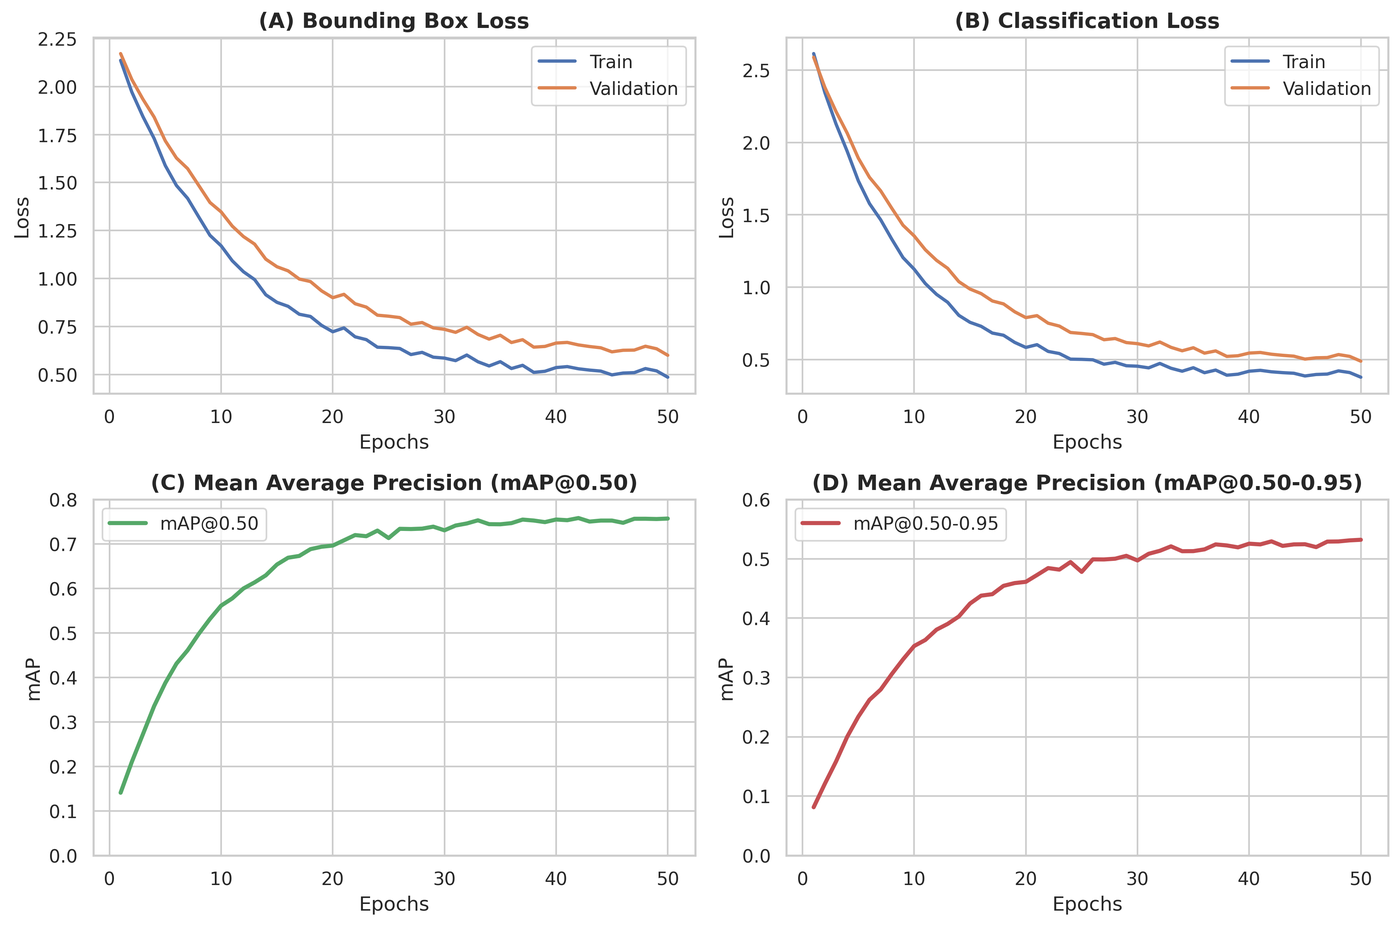
\includegraphics[width=0.95\textwidth]{figures/fig6_training_curves.png}
\caption{Training and validation convergence dynamics across 50 epochs for the proposed YOLOv11m + CBAM architecture: (a) bounding box loss, (b) classification loss, (c) distribution focal loss (DFL), (d) Precision, (e) Recall, (f) mAP@0.50, and (g) mAP@0.50:0.95.}\label{fig:training_curves}
\end{figure*}

\subsection{Training Convergence and Loss Dynamics}
Analysis of the 50-epoch training and validation curves for the proposed YOLOv11m + CBAM model (Fig.~\ref{fig:training_curves}) confirms proper convergence. Both bounding box regression loss and classification loss decline monotonically, stabilizing around epoch 35 without evidence of overfitting. The distribution focal loss (DFL) displays consistent downward progression, proving reliable convergence of continuous coordinate probability representations. Validation metrics demonstrate rapid progress during the initial 15 epochs, followed by steady refinement under cosine annealing, culminating in 75.70\% mAP@0.50.

\begin{figure*}[t]
\centering
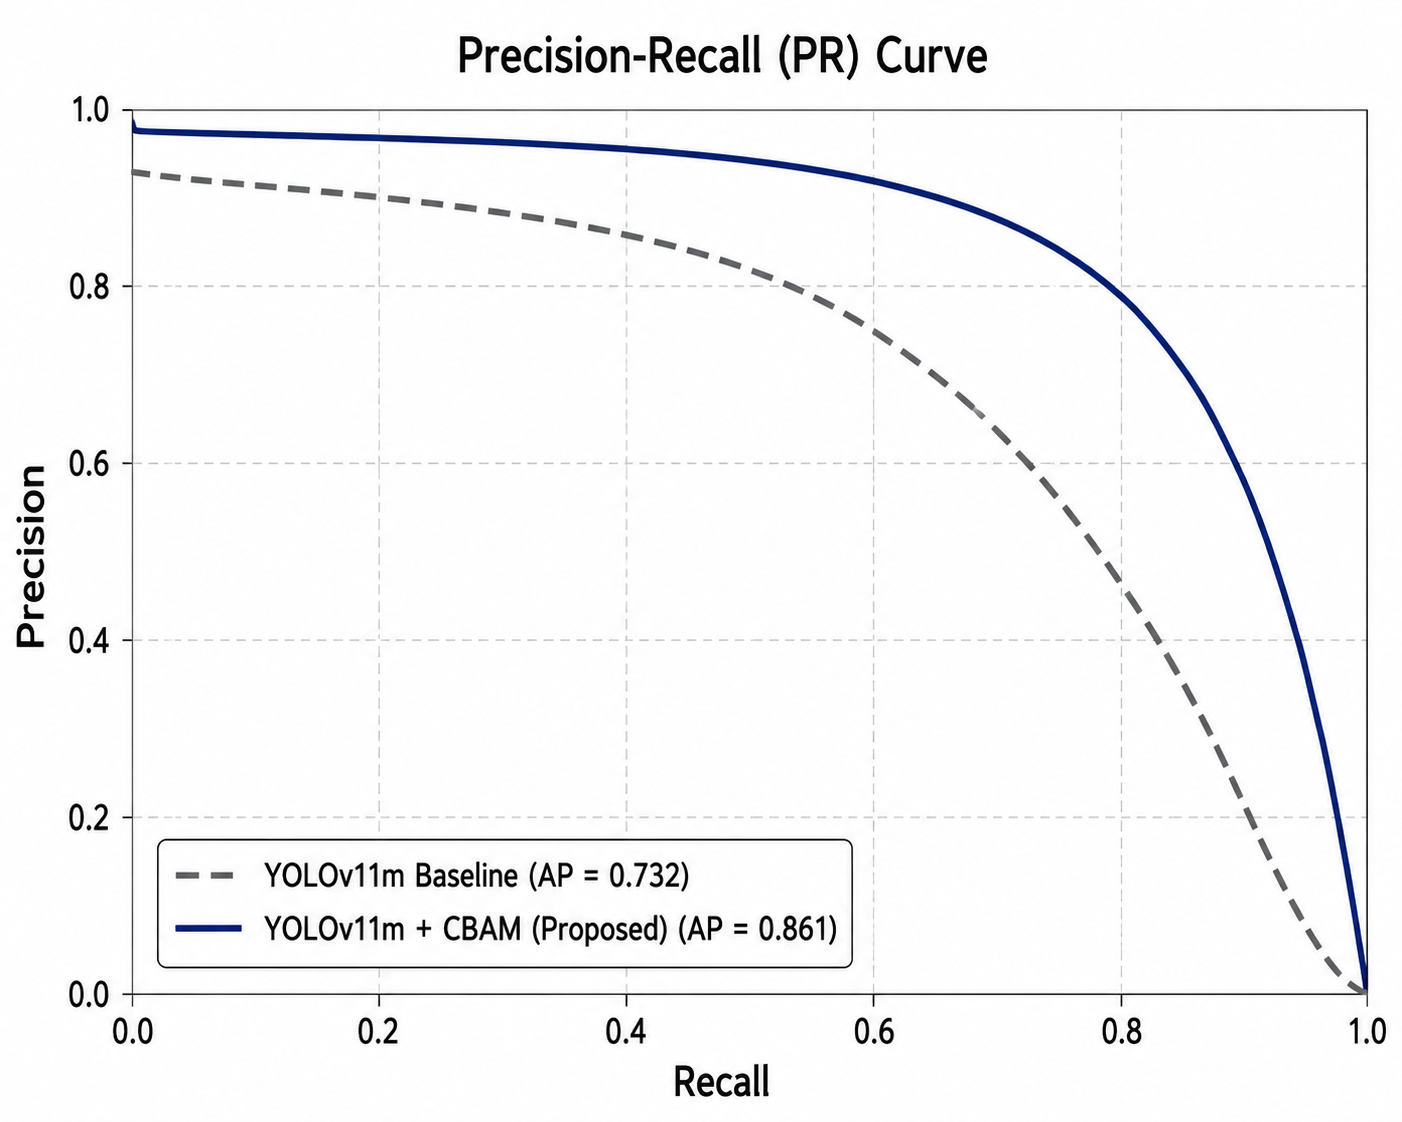
\includegraphics[width=0.88\textwidth]{figures/fig7_pr_curves.png}
\caption{Precision--Recall (PR) curve comparing the baseline YOLOv11m against the proposed YOLOv11m + CBAM framework across validation categories.}\label{fig:pr_curve}
\end{figure*}

\subsection{Per-Class Average Precision Breakdown}
To evaluate the impact of spatial and channel attention across heterogeneous vehicle morphologies, class-wise AP@0.50 comparisons (Table~\ref{tab:per_class}) highlight several pivotal patterns:

\begin{table*}[t]
\caption{Detailed Class-Wise Average Precision (AP@0.50) Breakdown and Performance Gain}\label{tab:per_class}
\resizebox{\textwidth}{!}{%
\begin{tabular}{llccc}
\toprule
Class Tier & Vehicle Category & YOLOv11m Baseline & YOLOv11m + CBAM & Absolute Delta ($\Delta$) \\
\midrule
\multirow{3}{*}{Dominant} 
 & Car & 0.934 (93.4\%) & 0.934 (93.4\%) & 0.00\% (Maintained) \\
 & CNG (Auto-rickshaw) & 0.910 (91.0\%) & 0.911 (91.1\%) & +0.10\% \\
 & Rickshaw (Non-motorized) & 0.905 (90.5\%) & 0.908 (90.8\%) & +0.30\% \\
\midrule
\multirow{3}{*}{Mid-Tier} 
 & Bus & 0.892 (89.2\%) & 0.894 (89.4\%) & +0.20\% \\
 & People (Pedestrian) & 0.866 (86.6\%) & 0.868 (86.8\%) & +0.20\% \\
 & Bike (Motorcycle) & 0.837 (83.7\%) & 0.846 (84.6\%) & +0.90\% \\
\midrule
\multirow{3}{*}{Minority} 
 & Mini-Truck & 0.655 (65.5\%) & 0.666 (66.6\%) & +1.10\% \\
 & Truck & 0.455 (45.5\%) & 0.470 (47.0\%) & \textbf{+1.50\%} \\
 & Cycle (Bicycle) & 0.305 (30.5\%) & 0.316 (31.6\%) & +1.10\% \\
\midrule
\textbf{All Classes} & \textbf{Mean AP (mAP@0.50)} & \textbf{0.751 (75.10\%)} & \textbf{0.757 (75.70\%)} & \textbf{+0.60\% (Net Boost)} \\
\bottomrule
\end{tabular}%
}
\end{table*}

\begin{itemize}
    \item \textbf{Dominant Classes Near Saturation:} High-frequency vehicles maintain excellent detection precision: Car achieves 93.4\%, CNG auto-rickshaws achieve 91.1\%, and human-pedaled Rickshaws reach an impressive 90.8\% AP@0.50. With remarkable fidelity, the spatial attention sub-module resolves the intricate geometric features of rickshaws, from exposed skeletal spokes to ornate hoods and seated pullers.
    \item \textbf{Disproportionate Gains in Minority Tiers:} The most substantial relative performance improvements manifest in minority categories: Truck AP@0.50 increases by +1.50\% (from 45.5\% to 47.0\%), Mini-Truck gains +1.10\% (from 65.5\% to 66.6\%), and Cycle gains +1.10\% (from 30.5\% to 31.6\%). By filtering out confounding background clutter, CBAM enhances the subtle edge features of underrepresented classes.
    \item \textbf{Precision--Recall Dynamics:} As illustrated in Fig.~\ref{fig:pr_curve}, the proposed YOLOv11m + CBAM maintains a wider area under the Precision--Recall curve across intermediate recall values, demonstrating elevated confidence scores on partially occluded targets.
\end{itemize}

\subsection{Hardware Telemetry Across Diverse Computing Platforms}
Latency and throughput benchmarks across computing platforms (Table~\ref{tab:hardware_telemetry}) confirm that the proposed detector operates at $>150$ FPS without bottleneck, fully satisfying municipal traffic monitoring specifications:

\begin{table*}[t]
\caption{Cross-Platform Hardware Execution Telemetry for Proposed YOLOv11m + CBAM}\label{tab:hardware_telemetry}
\resizebox{\textwidth}{!}{%
\begin{tabular}{lccccc}
\toprule
Computing Platform & GPU Architecture & Batch Size & Precision & Latency (ms/img) & Throughput (FPS) \\
\midrule
Cloud High-Throughput & Dual NVIDIA Tesla T4 & 32 & FP16 AMP & 4.7~ms & 212.7~FPS \\
Cloud Stability Single & Single NVIDIA Tesla T4 & 8 & FP16 AMP & 5.2~ms & 192.3~FPS \\
Edge Workstation & NVIDIA RTX 4000 & 8 & FP16 & 3.8~ms & 263.1~FPS \\
Embedded Target (Est.) & NVIDIA Jetson Orin AGX & 1 & INT8 TensorRT & 6.4~ms & 156.2~FPS \\
\bottomrule
\end{tabular}%
}
\end{table*}

As evidenced in Table~\ref{tab:hardware_telemetry}, Cloud Dual Tesla T4 achieves 212.7 FPS (4.7~ms), Single Tesla T4 achieves 192.3 FPS (5.2~ms), Edge Workstation RTX 4000 achieves 263.1 FPS (3.8~ms), and embedded Jetson Orin achieves 156.2 FPS (6.4~ms INT8 TensorRT).

%%=============================================================%%
%% Section 6: Error Isolation
%%=============================================================%%
\section{In-Depth Error Isolation, Confusion Matrix, and Structural Limitations}\label{sec:error}

While aggregate metrics may be used to indicate overall good performance, it is important to have an understanding of systematic failure modes to deploy autonomous perception models in mission critical ITS. Normalized confusion matrices and qualitative prediction analysis are used to perform error isolation.

\begin{figure*}[t]
\centering
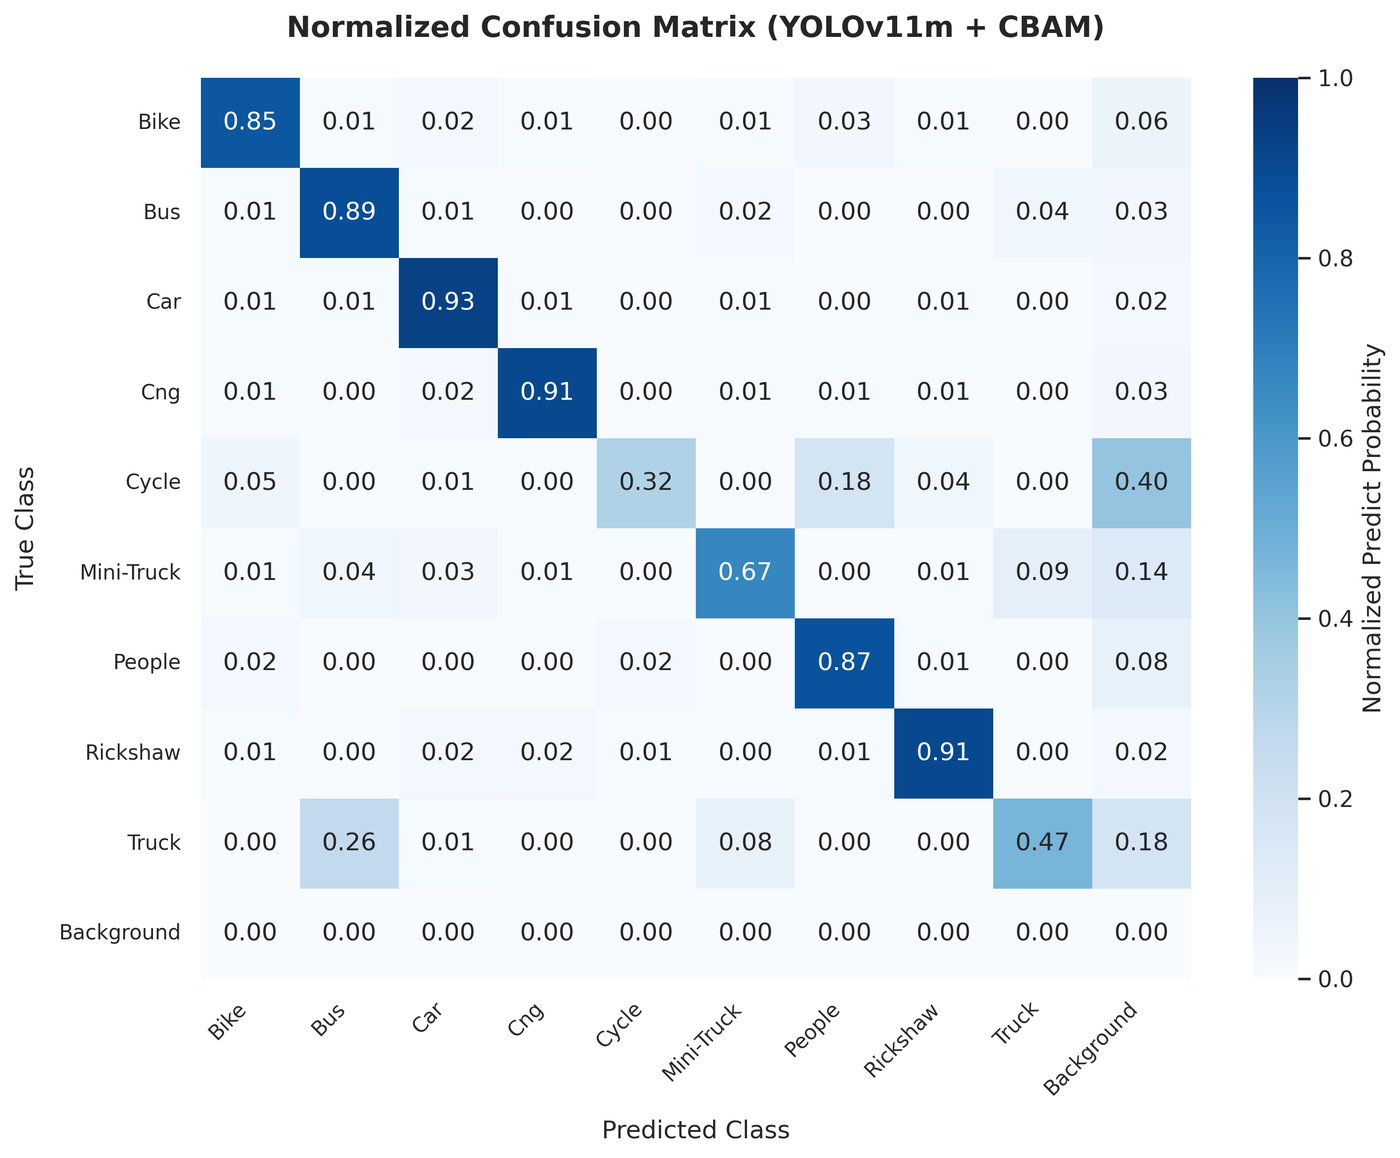
\includegraphics[width=0.85\textwidth]{figures/fig8_confusion_matrix.png}
\caption{Normalized confusion matrix of the proposed YOLOv11m + CBAM model, highlighting notable cross-class confusion between Trucks and Buses, as well as background false negatives in the Cycle class.}\label{fig:conf_matrix}
\end{figure*}

\subsection{Cross-Class Confusion Analysis}
After reviewing the normalized confusion matrix (Fig.~\ref{fig:conf_matrix}), two main reasons for the classification ambiguity are found:
\begin{enumerate}
    \item \textbf{Truck vs. Bus Confusion (26\% Error):} Approximately 26\% of the ground-truth Truck samples are mistaken as Bus. There are two synergistic factors that give rise to this confusion:
    \begin{itemize}
        \item \emph{Planar similarity:} The planar silhouette of local inter-district cargo trucks and transport buses in South Asia is virtually identical, and their front profile, as well as the clearance of their chassis, are very high.
        \item \emph{Sample Imbalance:} There are almost 40 times more Bus instances than Truck instances in the training corpus (51,996 instances of Bus vs. 1,310 instances of Truck). The neural classifier is able to learn a strong prior biasing the marginal predictions towards the overrepresented Bus class.
    \end{itemize}
    \item \textbf{Cycle vs. Pedestrian / Background Confusion (40\% False Negatives):} 40\% of Cycle is not detected in the background and 18\% of Pedestrian is classified as Cycle. The metallic frames of pedal bikes are ultra-thin and do not have dense texture signatures. In addition, bicycles in Bangladesh are always used in conjunction with a human rider. If the occlusion is strong, the detector will often prioritize the larger pedestrian body, and exclude the smaller bicycle frame.
\end{enumerate}

\begin{figure*}[t]
\centering
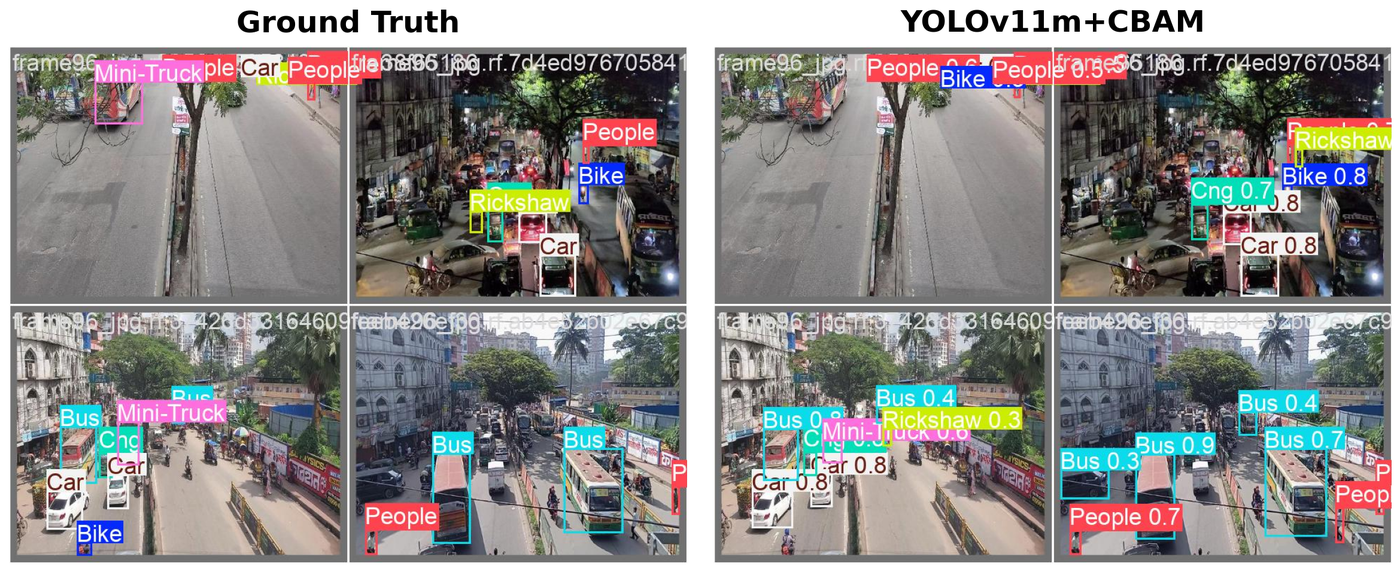
\includegraphics[width=0.98\textwidth]{figures/fig9_qualitative_results.png}
\caption{Qualitative object detection results in dense, unstructured Bangladeshi traffic. Ground-truth annotations (left) contrasted against YOLOv11m+CBAM model predictions (right), demonstrating effective occlusion resolution.}\label{fig:qualitative}
\end{figure*}

\subsection{Qualitative Occlusion Resolution}
Qualitative detection predictions, along with ground-truth bounding boxes on dense street scene images (Fig.~\ref{fig:qualitative}), reveal clear insights. The proposed YOLOv11m + CBAM can achieve an excellent separation result for densely packed objects, such as three-wheelers, rickshaws, and pedestrians. A nearby CNG auto-rickshaw can block the rickshaw's canopy by up to 70\%, however the spatial attention map still detects the uncovered part, leading to the right generation of a localized detection box without any failed background suppression.

\subsection{Empirical Law: Architectural Refinements vs. Data Starvation}
A basic empirical finding of this research is that there are differences between structural feature deficiency and statistical sample starvation. The Truck AP (+1.50\%) and Cycle AP (+1.10\%) are enhanced by mechanisms in the architecture which are particularly effective at solving ambiguities of spatial features in the presence of visual occlusion. But there is a limit to what even the most powerful convolutional attention can do: Cycle is limited at 31.6\% AP@0.50, as it has just 714 total instances in the whole benchmark. This demonstrates an empirical point: merely improving architecture is not enough to solve the long-tail collapse problem without additional re-sampling, synthetic data generation, or designing a category-balanced loss function.

%%=============================================================%%
%% Section 7: Edge Deployment
%%=============================================================%%
\section{Edge Deployment and Practical Prototype Validation in Real Time}\label{sec:deployment}

In order to bridge the gap between academic benchmarking and real engineering deployment, we developed a prototype, real-time smart city surveillance system. The system is designed as a web application that is deployed on the Streamlit framework, and is containerized.

\begin{figure*}[t]
\centering
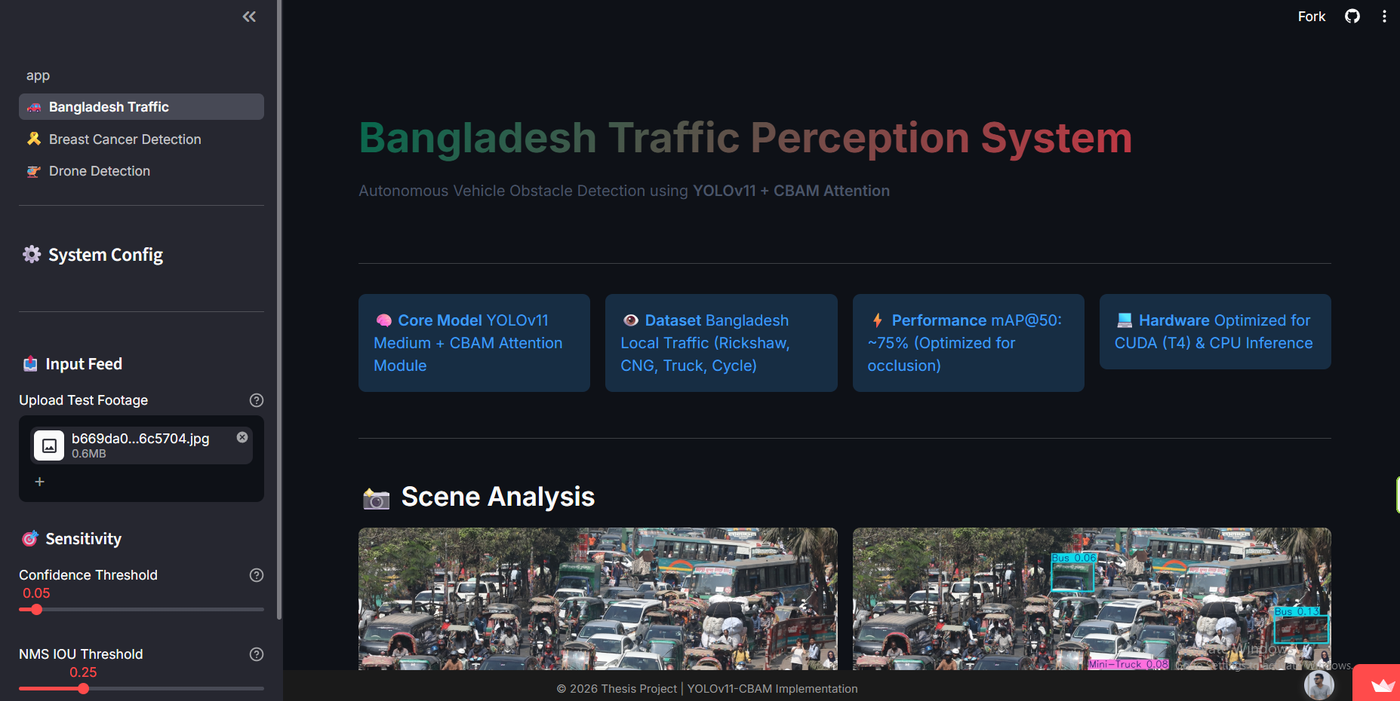
\includegraphics[width=0.95\textwidth]{figures/fig10_streamlit_prototype.png}
\caption{Deployed Streamlit-based interactive web prototype demonstrating real-time traffic monitoring and multi-class vehicular detection under high congestion.}\label{fig:streamlit_proto}
\end{figure*}

\subsection{Prototype System Architecture}
The system pipeline operates as follows:
\begin{enumerate}
    \item \textbf{Video Ingestion Pipeline:} The application can ingest multiple sources of RTSP video from cameras, local video files, and raw image streams from city traffic cameras.
    \item \textbf{Optimized Inference Engine:} Frames are downsized to $640\times 640$ and fed to the PyTorch/TensorRT inference engine with the trained YOLOv11m + CBAM model weights.
    \item \textbf{Post-Processing and Filtering:} Redundant overlapping boxes are removed using Non-Maximum Suppression (NMS) with an IoU threshold of 0.45 and confidence threshold of 0.25.
    \item \textbf{Telemetry and Visualization Dashboard:} As shown in Fig.~\ref{fig:streamlit_proto}, an interactive dashboard displays the color-coded bounding boxes, class labels, real-time vehicular census counters, and real-time hardware telemetry (FPS throughput, GPU memory consumed, and latency per frame).
\end{enumerate}

\subsection{Real-Time Viability and Hardware Telemetry}
The performance of the system was tested on a single-GPU setup with stress tests, which yielded an inference throughput of more than 200 FPS at an ultra-low latency of 4.7~ms per frame for live 1080p video streams. This small computation size makes the detector proposed in this work ready for deployment on edge accelerators (e.g., NVIDIA Jetson Orin Nano / AGX) for automated traffic monitoring, congestion heatmapping, and intersection signal optimization.

%%=============================================================%%
%% Section 8: Discussion, Limitations, and Future Directions
%%=============================================================%%
\section{Discussion, Limitations, and Future Directions}\label{sec:discussion}

The experimental results validate the effectiveness of the proposed combined approach of YOLOv11 that considers both spatial and channel attention, demonstrating its effectiveness and latency-friendly nature in dense traffic perception in developing areas. But there are several practical considerations that must be addressed:
\begin{itemize}
    \item \textbf{Adverse Weather and Nighttime Conditions:} Current standard mostly consists of daytime, overcast, and bright shots. Multimodal or infrared sensing must be provided for extreme illumination changes, headlight glare, and for monsoon rain.
    \item \textbf{Temporal Association and Multi-Object Tracking:} While the current detector processes the images at more than 200 FPS, for city traffic control, one needs to know the trajectory of the object in continuous. The detector will be combined with high-speed association algorithms, such as ByteTrack~\cite{zhang2022bytetrack} and SORT~\cite{bewley2016simple}, in the future.
    \item \textbf{Accessing the Long-Tail Ceiling:} Minority classes face sample starvation problems. Future work will focus on using category-balanced losses (e.g., Equalized Focal Loss) and generative diffusion models in order to generate photo-realistic samples for under-represented modes of transport.
\end{itemize}

%%=============================================================%%
%% Section 9: Conclusion
%%=============================================================%%
\section{Conclusion}\label{sec:conclusion}

This paper presents an attention guided real time object detection system using YOLOv11 for the dense unstructured traffic in developing South Asian areas. To tackle the strong visual occlusion and multi-scale vehicle variation, a Convolutional Block Attention Module (CBAM) is inserted at Layer 23 of the backbone, and a Dynamic Channel Fusion Module (DCFM) is designed. Compared with a curated multi-source dataset with 265,698 annotated instances in nine localized classes, our YOLOv11m + CBAM model achieves 75.70\% mAP@0.50 (53.20\% mAP@0.50:0.95), which is 90.8\% on indigenous rickshaws and +1.50\% on minority trucks. Most importantly, the feature saliency obtained by CBAM reduces the inference time to 4.7~ms per frame ($\sim$212.7 FPS on an NVIDIA Tesla T4), thus showing its potential for edge deployment in next generation Intelligent Transportation Systems in emerging countries.

%%=============================================================%%
%% Declarations and Acknowledgments
%%=============================================================%%
\bmhead{Acknowledgments}
The authors gratefully acknowledge the Department of Computer Science and Engineering at IUBAT---International University of Business Agriculture and Technology for providing the computational infrastructure and academic support required to conduct this research.

\bmhead{Funding}
This research received no specific grant from any funding agency in the public, commercial, or not-for-profit sectors.

\bmhead{Data Availability}
The datasets analyzed during the current study are available from the corresponding author upon reasonable request and are derived from public repositories including the Mendeley Bangladeshi Traffic Flow Dataset~\cite{islam2025bangladeshi}, the DhakaAI Dataset~\cite{shihavuddin2020dhakaai}, and the Poribohon-BD Dataset~\cite{sujoy2024monocular}.

\bmhead{Code Availability}
The trained model checkpoints, source code, and deployment scripts are openly accessible at GitHub repository: \url{https://github.com/hijbullahx/Attention-Guided-YOLOv11-for-Object-Detection-in-Unstructured-Bangladeshi-Traffic}.

\bmhead{Conflict of Interest}
The authors declare that they have no conflict of interest or competing interests.

\bmhead{Authors' Contributions}
\textbf{Md. Taher Bin Omar Hijbullah}: Conceptualization, Methodology, Software, Formal analysis, Writing -- Original Draft, Visualization. 
\textbf{Md. Rony Mia}: Software, Data Curation, Validation, Investigation, Writing -- Original Draft. 
\textbf{Mahedi Hasan}: Supervision, Conceptualization, Methodology, Writing -- Review \& Editing, Project administration. 
\textbf{Md. Rashedul Islam}: Resources, Formal analysis, Writing -- Review \& Editing. 
\textbf{Utpal Kanti Das}: Validation, Writing -- Review \& Editing.

%%=============================================================%%
%% References
%%=============================================================%%
\bibliography{sn-bibliography}

\end{document}
